\documentclass[11pt]{amsart}

\usepackage[T1]{fontenc}
\usepackage{lmodern}
\usepackage{amssymb,amsmath}
\usepackage{graphicx}
\usepackage{booktabs}
\usepackage{enumitem}
\usepackage[dvipsnames]{xcolor}
\usepackage[margin=1.15in]{geometry}
\usepackage[colorlinks=true,linkcolor=blue!50!black,citecolor=blue!50!black,urlcolor=blue!50!black]{hyperref}

\newtheorem{theorem}{Theorem}[section]
\newtheorem{proposition}[theorem]{Proposition}
\newtheorem{lemma}[theorem]{Lemma}
\newtheorem{corollary}[theorem]{Corollary}
\theoremstyle{definition}
\newtheorem{definition}[theorem]{Definition}
\theoremstyle{remark}
\newtheorem{remark}[theorem]{Remark}

\numberwithin{equation}{section}

\newcommand{\Z}{\mathbb{Z}}
\newcommand{\cw}{C_5[w]}
\newcommand{\lit}[1]{\mathsf{#1}}
\newcommand{\doi}[1]{\href{https://doi.org/#1}{\nolinkurl{doi:#1}}}
\hypersetup{pdftitle={The biplanar clique blow-ups of the five-cycle},pdfauthor={Deep Bhattacharjee}}

\begin{document}

\title{The biplanar clique blow-ups of the five-cycle}

\author{Deep Bhattacharjee}
\address{Formerly, Electro-Gravitational Space Propulsion Laboratory (EGSPL),\newline Bhubaneswar, Odisha 751030, India}
\email{d.bhattacharjee@erl-forschung.de}
\email{itsdeep@live.com}
\urladdr{https://orcid.org/0000-0003-0466-750X}
\thanks{Corresponding author: \href{mailto:d.bhattacharjee@erl-forschung.de}{d.bhattacharjee@erl-forschung.de}; ORCID \href{https://orcid.org/0000-0003-0466-750X}{\mbox{0000-0003-0466-750X}}}

\subjclass[2020]{Primary 05C10; Secondary 05C15, 05C83}
\keywords{Earth--Moon problem, thickness, biplanar graph, clique blow-up, Schnyder's theorem, LRAT}

\begin{abstract}
We prove that a clique blow-up of the five-cycle is biplanar if and only if it has at most sixteen vertices and clique number at most eight. Consequently every biplanar clique blow-up of the five-cycle is $8$-colourable, which answers a question of Trivedi. The non-biplanar cases are refuted by a propositional encoding of biplanarity, strengthened by a contraction argument for $K_9$, whose unsatisfiability certificates are checked in Lean~4.
\end{abstract}

\maketitle

\section{Introduction}

A graph is \emph{biplanar} if its edge set is the union of the edge sets of two planar graphs on the same vertex set. Ringel's Earth--Moon problem~\cite{Ri} asks for the largest chromatic number of a biplanar graph. A biplanar graph on $n\ge 3$ vertices has at most $6n-12$ edges, so biplanar graphs are $11$-degenerate and $12$ colours always suffice; Sulanke's graph, the join of a five-cycle with $K_6$, is biplanar and $9$-chromatic~\cite{Ga,Hu}. The answer is known only to lie in $\{9,10,11,12\}$~\cite{Ge}.

Graphs of small independence number are the natural candidates for large chromatic number, and clique blow-ups of odd cycles are the simplest of them. For $w=(w_1,\dots,w_5)\in\Z_{\ge1}^5$ let $\cw$ be the graph whose vertex set is the disjoint union of \emph{bags} $A_1,\dots,A_5$ with $|A_i|=w_i$, two distinct vertices being adjacent when their bags are equal or consecutive on the five-cycle. Indices of bags are read modulo~$5$ throughout, and we write
\[
n(w)=w_1+\dots+w_5,\qquad s(w)=\max_{1\le i\le5}\,(w_i+w_{i+1}).
\]
Thus $n(w)$ is the number of vertices of $\cw$ and $s(w)$ its clique number. Every independent set of $\cw$ meets at most two bags, so $\chi(\cw)\ge\lceil n(w)/2\rceil$. Boutin, Gethner and Sulanke proved that the blow-ups $C_m[K_3]$ are biplanar for every $m\ge4$~\cite{BGS}, and Albertson, Boutin and Gethner asked about thickness and chromatic number of unbalanced blow-ups~\cite{ABG}. Trivedi~\cite{Tr} showed that
\begin{equation}\label{eq:chi}
\chi(\cw)=\max\bigl\{s(w),\,\lceil n(w)/2\rceil\bigr\},
\end{equation}
deduced that every biplanar $\cw$ is $9$-colourable, and asked whether the value $9$ is attained~\cite[Question~7.3]{Tr}. By~\eqref{eq:chi} this happens only for $n(w)\in\{17,18\}$, and he reduced the question to $35$ weight vectors. Kirchweger, Scheucher and Szeider had earlier shown with a long SAT computation that $C_5[4,4,4,4,3]$ is not biplanar~\cite{KSS}, and Szeider has since proved that every biplanar graph of independence number at most two has at most eighteen vertices and is $9$-colourable~\cite{Sz}. Since $9$-chromatic biplanar graphs of independence number two exist on seventeen vertices~\cite{GS}, neither result decides Trivedi's question.

\begin{theorem}\label{thm:main}
Let $w\in\Z_{\ge1}^5$. The graph $\cw$ is biplanar if and only if $s(w)\le8$ and $n(w)\le16$.
\end{theorem}

\begin{corollary}\label{cor:chi}
Every biplanar clique blow-up of the five-cycle is $8$-colourable, and the bound is attained by the biplanar graph $C_5[3,3,3,3,4]$. In particular no biplanar clique blow-up of the five-cycle is $9$-chromatic, and Question~7.3 of~\cite{Tr} has a negative answer.
\end{corollary}

\begin{proof}
If $\cw$ is biplanar then $s(w)\le8$ and $n(w)\le16$ by Theorem~\ref{thm:main}, so $\chi(\cw)\le8$ by~\eqref{eq:chi}. The graph $C_5[3,3,3,3,4]$ satisfies both conditions and has sixteen vertices, so it is biplanar and $\chi\ge\lceil 16/2\rceil=8$.
\end{proof}

The condition $s(w)\le8$ is necessary because two consecutive bags span a clique of order $w_i+w_{i+1}$, and $K_9$ is not biplanar~\cite{BHK,Tu}. Section~\ref{sec:reduction} reduces the rest of Theorem~\ref{thm:main} to $36$ graphs on sixteen vertices, which we draw, and $26$ graphs on seventeen vertices, which we refute. A biplanar graph on seventeen vertices has at most $90$ edges while ours have between $71$ and $80$, so counting gives nothing, and a direct search over pairs of planar graphs is hopeless. The refutation rests on Lemma~\ref{lem:contract}: if a component of one layer outside an $8$-clique $Q$ sees enough of $Q$, contracting it produces a ninth vertex adjacent to all of $Q$, and the two layers then contain $K_9$. Section~\ref{sec:encoding} builds this into a propositional formula, and Section~\ref{sec:certificates} describes the unsatisfiability certificates and how they are checked.\footnote{The drawings, the colourings, the reduction to finitely many weight vectors and all $26$ unsatisfiability certificates are checked in Lean~4; Section~\ref{sec:certificates} lists what is checked and what is assumed.}

\section{Reduction to finitely many graphs}\label{sec:reduction}

The dihedral group of the five-cycle acts on $\Z_{\ge1}^5$ by permuting coordinates, and $\cw$ depends on $w$ only up to this action. If $v\le w$ coordinatewise then $C_5[v]$ is an induced subgraph of $\cw$, and subgraphs of biplanar graphs are biplanar.

\begin{lemma}\label{lem:reduce}
Let $w\in\Z_{\ge1}^5$ with $s(w)\le8$.
\begin{enumerate}[label=\textup{(\alph*)}]
\item If $n(w)\ge17$, there is $v\in\Z_{\ge1}^5$ with $v\le w$, $n(v)=17$ and $s(v)\le8$.
\item If $n(w)\le16$, there is $v\in\Z_{\ge1}^5$ with $v\ge w$, $n(v)=16$ and $s(v)\le8$.
\end{enumerate}
\end{lemma}

\begin{proof}
(a) While $n(w)>17$ some coordinate is at least $2$; lowering it by one keeps all coordinates positive and does not increase $s$.

(b) Call the pair $\{i,i+1\}$ \emph{tight} if $w_i+w_{i+1}=8$. If no coordinate can be raised by one without breaking $s(w)\le8$, every $i$ lies in a tight pair. The five-cycle has no three pairwise intersecting edges, so a set of edges covering all five vertices contains two disjoint ones, say $\{i,i+1\}$ and $\{i+2,i+3\}$; then $n(w)=8+8+w_{i+4}\ge17$. Hence when $n(w)\le16$ some coordinate can be raised, and we repeat until $n=16$.
\end{proof}

Listing the vectors directly gives the following.

\begin{lemma}\label{lem:lists}
Up to the dihedral action there are exactly $26$ vectors $w\in\Z_{\ge1}^5$ with $n(w)=17$ and $s(w)\le8$, and exactly $36$ with $n(w)=16$ and $s(w)\le8$. They are listed in Tables~\ref{tab:certs} and~\ref{tab:sixteen}.
\end{lemma}

Since $s(w)\le8$ and all coordinates are positive, every coordinate is at most $7$, so the lists come from a finite enumeration. The $26$ vectors of the first list all satisfy Trivedi's further conditions $\sum_i w_iw_{i+1}\le4n-8$ and $e\le6n-12$, and they are exactly his seventeen-vertex candidates; his nine eighteen-vertex candidates each contain one of them.

\begin{table}[ht]
\centering\small
\begin{tabular}{cccccc}
\toprule
$1,1,6,1,7$ & $1,1,6,2,6$ & $1,2,5,1,7$ & $1,2,5,2,6$ & $1,2,5,3,5$ & $1,2,6,1,6$\\
$1,2,6,2,5$ & $1,3,4,1,7$ & $1,3,4,2,6$ & $1,3,4,3,5$ & $1,3,4,4,4$ & $1,3,5,1,6$\\
$1,3,5,2,5$ & $1,3,5,3,4$ & $1,4,3,2,6$ & $1,4,3,3,5$ & $1,4,3,4,4$ & $1,4,4,1,6$\\
$1,4,4,2,5$ & $1,5,2,2,6$ & $1,5,2,3,5$ & $2,2,4,2,6$ & $2,2,4,3,5$ & $2,2,4,4,4$\\
$2,2,5,2,5$ & $2,3,3,2,6$ & $2,3,3,3,5$ & $2,3,3,4,4$ & $2,3,3,5,3$ & $2,3,4,2,5$\\
$2,3,4,3,4$ & $2,3,4,4,3$ & $2,3,5,2,4$ & $2,4,2,4,4$ & $2,4,3,3,4$ & $3,3,3,3,4$\\
\bottomrule
\end{tabular}
\caption{The $36$ weight vectors with $n(w)=16$ and $s(w)\le8$, up to the dihedral action. For each of them $\cw$ is the union of two planar graphs with explicit straight-line drawings.}\label{tab:sixteen}
\end{table}

\begin{proposition}\label{prop:sixteen}
For each of the $36$ vectors of Table~\ref{tab:sixteen}, the graph $\cw$ is biplanar.
\end{proposition}

\begin{proof}
For each vector we give two edge sets $L_1,L_2$ with $L_1\cup L_2=E(\cw)$ and, for each $L_j$, an injective placement of the sixteen vertices at lattice points of $[0,28]\times[0,14]$ such that no vertex lies on a segment between two others joined in $L_j$ and no two segments of $L_j$ without a common endpoint meet. Each $L_j$ is then a plane straight-line drawing. The data are part of the archive~\cite{Ar}; every condition is a sign test on a $2\times2$ integer determinant. Figure~\ref{fig:layers} shows a redrawing of the two layers for $w=(3,3,3,3,4)$.
\end{proof}

\begin{figure}[ht]
\centering
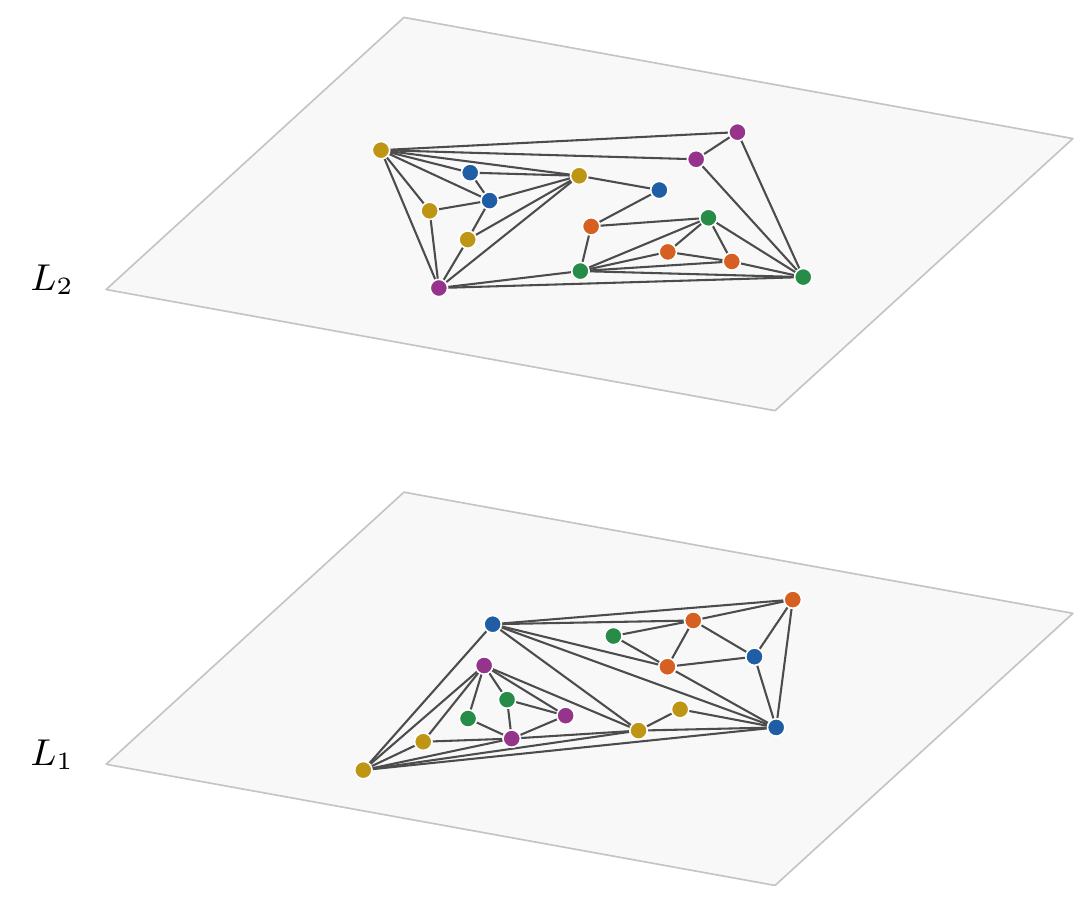
\includegraphics[width=0.62\textwidth]{figures/layers.png}
\caption{The two planar layers $L_1$ and $L_2$ of $C_5[3,3,3,3,4]$. Vertices are coloured by bag; every edge of the graph lies in one of the two layers.}\label{fig:layers}
\end{figure}

\section{A contraction lemma for \texorpdfstring{$K_9$}{K9}}\label{sec:contraction}

From now on $G$ is a graph whose edge set is $E(L_1)\cup E(L_2)$ for two planar graphs $L_1,L_2$ on $V(G)$, its \emph{layers}. For $S\subseteq V(G)$ we write $L_j[S]$ for the induced subgraph, and for a set $C$ of vertices $N_j(C)$ is the set of vertices outside $C$ with an $L_j$-neighbour in $C$.

\begin{lemma}\label{lem:contract}
Let $Q$ be a clique of $G$ with $|Q|=8$ and put $W=V(G)\setminus Q$. For $j=1,2$ let $C_j$ be either empty or the vertex set of a component of $L_j[W]$, and let $F_j\subseteq Q$ contain at most one vertex from each component of $L_j[Q]$ that is disjoint from $N_j(C_j)$. Then
\[
\bigl(N_1(C_1)\cup F_1\bigr)\cup\bigl(N_2(C_2)\cup F_2\bigr)\ne Q .
\]
\end{lemma}

\begin{proof}
Suppose the union is $Q$. Fix $j$. If $C_j\neq\emptyset$, contract the connected set $C_j$ of $L_j[Q\cup C_j]$ to a single vertex $z$; if $C_j=\emptyset$, add an isolated vertex $z$ to $L_j[Q]$. The result $H_j$ is planar, as a minor of $L_j$, and $z$ is adjacent in $H_j$ exactly to $N_j(C_j)\cap Q=N_j(C_j)$.\footnote{Every neighbour of a component of $L_j[W]$ lies in $Q$, since another neighbour in $W$ would belong to the component.} A component $K$ of $L_j[Q]$ disjoint from $N_j(C_j)$ has no edge to $z$, so it is a component of $H_j$ not containing $z$. Joining $z$ to one vertex of such a component keeps the graph planar: draw $K$ inside a face incident with $z$, with the chosen vertex on the outer face of $K$. Doing this for the components that meet $F_j$, one at a time, gives a planar graph $H_j'$ on $Q\cup\{z\}$ in which $z$ is adjacent to $N_j(C_j)\cup F_j$; a component already joined to $z$ is never used twice, since $F_j$ has at most one vertex in it. Figure~\ref{fig:contract} shows the construction.

Every edge of the clique $Q$ lies in $L_1$ or in $L_2$, hence in $L_1[Q]\subseteq H_1'$ or in $L_2[Q]\subseteq H_2'$, and $z$ is adjacent to every vertex of $Q$ in $H_1'$ or in $H_2'$ by assumption. So $H_1'\cup H_2'$ contains a $K_9$ on $Q\cup\{z\}$ and is the union of two planar graphs, contradicting the theorem of Battle, Harary and Kodama and of Tutte~\cite{BHK,Tu}.
\end{proof}

\begin{figure}[ht]
\centering
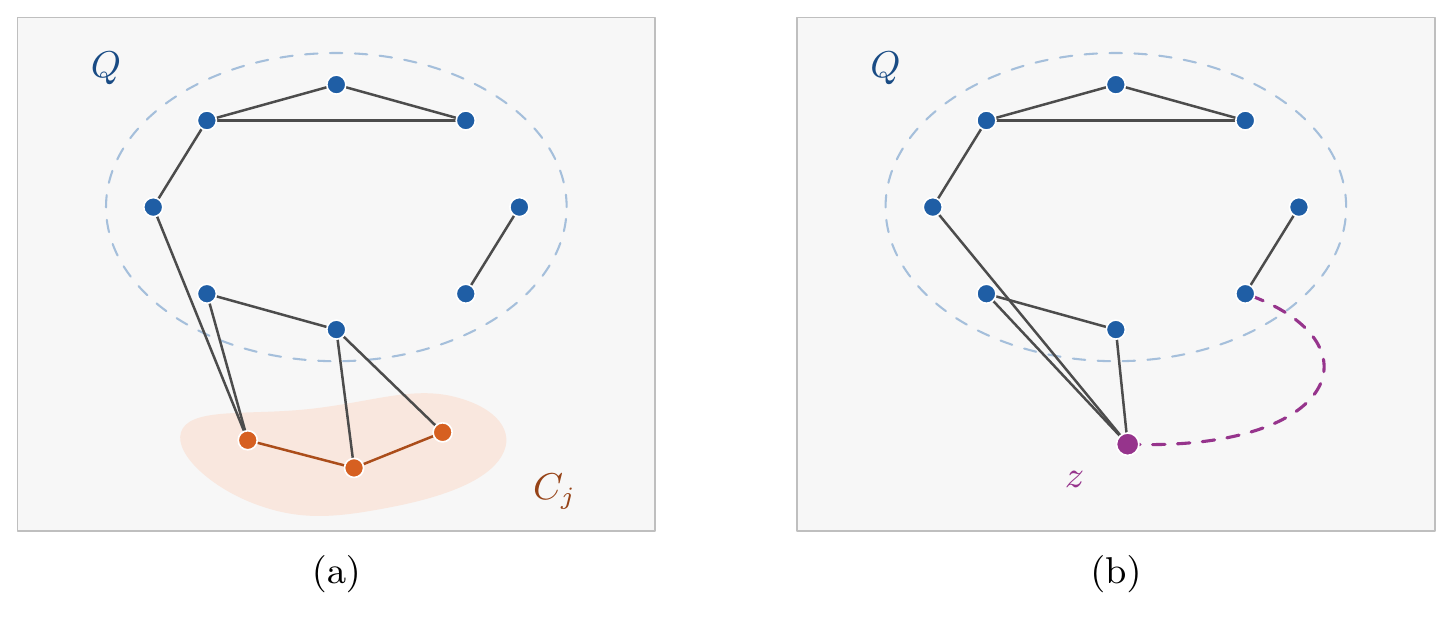
\includegraphics[width=0.86\textwidth]{figures/contraction.png}
\caption{Lemma~\ref{lem:contract} in one layer. (a) A component $C_j$ of $L_j[W]$ and its neighbours in the clique $Q$. (b) After contraction $z$ is adjacent to $N_j(C_j)$; the dashed edge joins $z$ to a component of $L_j[Q]$ that $C_j$ does not reach, and keeps the layer planar.}\label{fig:contract}
\end{figure}

In $\cw$ with $s(w)\le 8$, each pair of consecutive bags with $w_i+w_{i+1}=8$ is such a clique $Q$, and $W$ is the union of the other three bags.

\section{The encoding}\label{sec:encoding}

We use Schnyder's characterisation of planarity in the following form.

\begin{theorem}[Schnyder~\cite{Sc}]\label{thm:schnyder}
If a graph $H$ is planar, there are three linear orders $<_1,<_2,<_3$ on $V(H)$ such that for every edge $uv$ and every vertex $x\notin\{u,v\}$ there is an $i$ with $u<_ix$ and $v<_ix$.
\end{theorem}

Schnyder proved that the incidence poset of vertices and edges of a planar graph has dimension at most three. Restricting a realizer to the vertices gives the orders above: an edge $e=uv$ and a vertex $x\notin e$ are incomparable, so some linear extension puts $x$ above $e$ and hence above $u$ and $v$.\footnote{The converse also holds, but it is not used: the biplanar graphs of Proposition~\ref{prop:sixteen} are certified by drawings.} The same condition is the planarity encoding used in~\cite{KSS}.

Fix $w$ with $n=n(w)$, number the vertices $0,\dots,n-1$ bag by bag, and let $E$ be the edge set of $\cw$. The formula $\Phi(w)$ has the following variables: $o^{j,i}_{ab}$ for $j\in\{1,2\}$, $i\in\{1,2,3\}$ and $a<b$, meaning $a<_{j,i}b$ in the $i$th order of layer $j$ (with $o^{j,i}_{ba}$ standing for $\neg o^{j,i}_{ab}$); $\ell^j_e$ for $e\in E$, meaning $e\in L_j$; and auxiliary variables, each defined by a conjunction or disjunction of earlier literals through the usual three-clause definitions~\cite{Ts}. Its clauses are:
\begin{enumerate}[label=\textup{(E\arabic*)},leftmargin=*]
\item transitivity of each order $<_{j,i}$;
\item $\ell^1_e\vee\ell^2_e$ for every $e\in E$;
\item for every $e=uv\in E$, every $j$ and every $x\notin\{u,v\}$: $\ell^j_e\Rightarrow\bigvee_{i}\bigl(o^{j,i}_{ux}\wedge o^{j,i}_{vx}\bigr)$;
\item for any two vertices $a<b$ that are consecutive in the numbering of the same bag, $a<_{1,1}b$;
\item the clauses of Lemma~\ref{lem:contract} described below, for every pair of consecutive bags $Q=A_i\cup A_{i+1}$ with $|Q|=8$;
\item for every $j$ and every subgraph $S$ of $\cw$ isomorphic to $K_5$ or $K_{3,3}$, the clause $\bigvee_{e\in E(S)}\neg\ell^j_e$; and for every $j$ and every clique $S$ of $\cw$ with $s\in\{6,7,8\}$ vertices, the constraint that at most $3s-6$ of the variables $\ell^j_e$ with $e\subseteq S$ are true, written with the sequential counter of~\cite{Si}.
\end{enumerate}

For (E5) fix such a $Q$ and $W=V\setminus Q$. Connectivity inside a set $S$ is expressed by the variables
\[
r^{j,S,0}_{xy}=[x=y],\qquad r^{j,S,t+1}_{xy}=r^{j,S,t}_{xy}\vee\bigvee_{z\in S,\ zy\in E}\bigl(r^{j,S,t}_{xz}\wedge\ell^j_{zy}\bigr),
\]
and $R^{j,S}_{xy}=r^{j,S,|S|-1}_{xy}$ holds exactly when $x$ and $y$ lie in one component of $L_j[S]$. For $x\in W\cup\{\ast\}$ and $q\in Q$ put
\[
\lit{att}^j_{x,q}=\bigvee_{y\in W,\ yq\in E}\bigl(R^{j,W}_{xy}\wedge\ell^j_{yq}\bigr),\qquad \lit{att}^j_{\ast,q}=\bot,\qquad
\lit{free}^j_{x,u}=\bigwedge_{q\in Q}\neg\bigl(R^{j,Q}_{uq}\wedge\lit{att}^j_{x,q}\bigr).
\]
So $\lit{att}^j_{x,q}$ says that $q\in N_j(C)$ for the component $C$ of $x$ in $L_j[W]$ (with $C=\emptyset$ for $x=\ast$), and $\lit{free}^j_{x,u}$ that the component of $u$ in $L_j[Q]$ is disjoint from $N_j(C)$. For every pair $x_1,x_2\in W\cup\{\ast\}$ let $c_q=\lit{att}^1_{x_1,q}\vee\lit{att}^2_{x_2,q}$, and for $T\subseteq Q$ write $c_{Q\setminus T}$ for $\bigwedge_{q\in Q\setminus T}c_q$. The clauses (E5) forbid
\begin{align*}
&c_Q; \qquad c_{Q\setminus\{u\}}\wedge\lit{free}^j_{x_j,u}\quad(u\in Q,\ j=1,2);\qquad
c_{Q\setminus\{u,u'\}}\wedge\lit{free}^1_{x_1,u}\wedge\lit{free}^2_{x_2,u'}\quad(u\ne u');\\
&c_{Q\setminus\{u,u'\}}\wedge\lit{free}^j_{x_j,u}\wedge\lit{free}^j_{x_j,u'}\wedge\neg R^{j,Q}_{uu'}\quad(u\ne u',\ j=1,2).
\end{align*}

\begin{proposition}\label{prop:sound}
If $\cw$ is biplanar, then $\Phi(w)$ is satisfiable.
\end{proposition}

\begin{proof}
Let $L_1,L_2$ be planar layers of $\cw$. Every permutation of a bag is an automorphism of $\cw$, so after renaming the vertices inside each bag we may assume that the orders of Theorem~\ref{thm:schnyder} for $L_1$ list each bag in increasing order in $<_{1,1}$; renaming carries layers to layers and orders to orders. Set $\ell^j_e$ true exactly when $e\in E(L_j)$, the variables $o$ from the six orders, and every auxiliary variable to the value of its definition. Then (E1), (E2) and (E4) hold, and (E3) holds by Theorem~\ref{thm:schnyder}. A planar graph contains neither $K_5$ nor $K_{3,3}$~\cite{Ku}, and a planar graph on $s\ge3$ vertices has at most $3s-6$ edges, so the edges of $L_j$ inside a clique of $s$ vertices number at most $3s-6$; with the counter variables set to their intended values, (E6) holds.

By induction on $t$, $r^{j,S,t}_{xy}$ is true exactly when $L_j[S]$ has an $x$--$y$ walk of length at most $t$, so $R^{j,S}_{xy}$ is reachability in $L_j[S]$, and $\lit{att}$ and $\lit{free}$ have the meaning stated above. Given $x_1,x_2$, let $C_j$ be the component of $x_j$ in $L_j[W]$, or $\emptyset$ if $x_j=\ast$. Then $c_q$ is true exactly when $q\in N_1(C_1)\cup N_2(C_2)$. A violated clause of (E5) would give sets $F_1,F_2$ with at most two elements in total, each element in a component of $L_j[Q]$ disjoint from $N_j(C_j)$ and two elements of $F_j$ in different components, such that $N_1(C_1)\cup F_1\cup N_2(C_2)\cup F_2=Q$. Lemma~\ref{lem:contract} rules this out.
\end{proof}

The formula carries one clause family for each $8$-clique and each pair $x_1,x_2$, and only covers with at most two added edges; that is all the computation needed. The variables $o^{j,i}_{ab}$ are indexed arithmetically, so some indices do not occur.

\section{Certificates}\label{sec:certificates}

\begin{theorem}\label{thm:unsat}
For each of the $26$ vectors $w$ of Table~\ref{tab:certs}, $\Phi(w)$ is unsatisfiable. Hence none of the graphs $\cw$ is biplanar.
\end{theorem}

The formulas are produced by a Lean~4 function from $w$, and the clause counts in Table~\ref{tab:certs} are those of its output. CaDiCaL~3.0.1~\cite{CaD} refutes each formula on one core and writes a proof in the LRAT format~\cite{LRAT}, a clausal proof in which every derived clause carries the hints that justify it. The proofs were shortened with lrat-trim, which keeps only the clauses used in the final refutation, and each trimmed proof was then checked against the formula by the LRAT checker of the Lean~4 standard library~\cite{Le}, which is proved sound in Lean. The result of each check is a Lean theorem stating that the formula is unsatisfiable.

\begin{table}[ht]
\centering\small
%TABLE_CERTS%
\caption{The $26$ weight vectors with $n(w)=17$ and $s(w)\le8$, up to the dihedral action, with the size of $\Phi(w)$, the solving time of CaDiCaL, the size of the trimmed LRAT proof and the time of the Lean check.}\label{tab:certs}
\end{table}

The argument rests on the following, which are not formalised: Theorem~\ref{thm:schnyder}; the non-planarity of $K_5$ and $K_{3,3}$ and the bound $3s-6$ for planar graphs on $s\ge3$ vertices; the facts that minors of planar graphs are planar and that joining two components of a planar graph by an edge keeps it planar; the non-biplanarity of $K_9$~\cite{BHK,Tu}; and Proposition~\ref{prop:sound}, whose proof is above. The Lean checks of the certificates evaluate the verified checker by compiled code, so they also trust the Lean compiler. Proposition~\ref{prop:sixteen}, Lemma~\ref{lem:lists}, the enumeration behind Lemma~\ref{lem:reduce} and $8$-colourings of the $36$ graphs of Table~\ref{tab:sixteen} are checked in Lean by kernel evaluation.\footnote{The colourings give a second proof of the bound $\chi\le8$ in Corollary~\ref{cor:chi} that does not use~\eqref{eq:chi}: a biplanar $\cw$ is a subgraph of one of the $36$ graphs.}

\section{Proof of Theorem~\ref{thm:main}}\label{sec:proof}

Let $w\in\Z_{\ge1}^5$. If $s(w)\ge9$ then $\cw$ contains $K_9$ and is not biplanar. Suppose $s(w)\le8$. If $n(w)\ge17$, Lemma~\ref{lem:reduce}(a) gives $v\le w$ with $n(v)=17$ and $s(v)\le8$; up to symmetry $v$ is in Table~\ref{tab:certs}, so $C_5[v]$ is not biplanar by Theorem~\ref{thm:unsat}, and neither is its supergraph $\cw$. If $n(w)\le16$, Lemma~\ref{lem:reduce}(b) gives $v\ge w$ in Table~\ref{tab:sixteen} up to symmetry, and $\cw$ is a subgraph of the biplanar graph $C_5[v]$ of Proposition~\ref{prop:sixteen}. \qed

\begin{remark}
The graph $C_5[4,4,4,4,3]$ of~\cite{KSS} contains $C_5[3,3,3,4,4]$, one of the graphs of Table~\ref{tab:certs}. The clauses (E5) are what make the computation feasible: without them CaDiCaL did not refute the formula for $w=(1,1,7,1,7)$, the easiest of the $26$, within thirty minutes, while with them it is refuted in under a minute and the slowest of the $26$ takes %SLOWEST%. The contraction clauses are useful whenever a graph has many $8$-cliques whose complements are small.
\end{remark}

\subsection*{Data availability}
The weight vectors, drawings, colourings, formulas and certificates, together with the Lean~4 development and independent checks, are archived with the source of this paper~\cite{Ar}.

\subsection*{Use of generative AI}
During the preparation of this work the author used Claude (Anthropic) to search the literature, to run and check the computations, and to draft the text. The author checked every step of the proofs and every reference, and takes full responsibility for the content.

\begin{thebibliography}{99}

\bibitem{ABG}
M.~O. Albertson, D.~L. Boutin and E.~Gethner, \emph{The thickness and chromatic number of $r$-inflated graphs}, Discrete Math. \textbf{310} (2010), 2725--2734.

\bibitem{Ar}
D.~Bhattacharjee, \emph{The biplanar clique blow-ups of the five-cycle: paper, Lean~4 development and certificates}, Zenodo, 2026. %ARCHIVE%

\bibitem{BHK}
J.~Battle, F.~Harary and Y.~Kodama, \emph{Every planar graph with nine points has a nonplanar complement}, Bull. Amer. Math. Soc. \textbf{68} (1962), 569--571. \doi{10.1090/S0002-9904-1962-10850-7}

\bibitem{BGS}
D.~L. Boutin, E.~Gethner and T.~Sulanke, \emph{Thickness-two graphs part one: new nine-critical graphs, permuted layer graphs, and Catlin's graphs}, J. Graph Theory \textbf{57} (2008), 198--214. \doi{10.1002/jgt.20282}

\bibitem{CaD}
A.~Biere, T.~Faller, K.~Fazekas, M.~Fleury, N.~Froleyks and F.~Pollitt, \emph{CaDiCaL 2.0}, in: Computer Aided Verification (CAV 2024), Lecture Notes in Comput. Sci. \textbf{14681}, Springer, 2024, 133--152. \doi{10.1007/978-3-031-65627-9_7}

\bibitem{LRAT}
L.~Cruz-Filipe, M.~J.~H. Heule, W.~A. Hunt, M.~Kaufmann and P.~Schneider-Kamp, \emph{Efficient certified RAT verification}, in: Automated Deduction (CADE 26), Lecture Notes in Comput. Sci. \textbf{10395}, Springer, 2017, 220--236. \doi{10.1007/978-3-319-63046-5_14}

\bibitem{Ga}
M.~Gardner, \emph{Mathematical games}, Scientific American \textbf{242}(2) (1980), 14--23. \doi{10.1038/scientificamerican0280-14}

\bibitem{Ge}
E.~Gethner, \emph{To the Moon and beyond}, in: Graph Theory: Favorite Conjectures and Open Problems~2, Problem Books in Mathematics, Springer, 2018, 115--133. \doi{10.1007/978-3-319-97686-0_11}

\bibitem{GS}
E.~Gethner and T.~Sulanke, \emph{Thickness-two graphs part two: more new nine-critical graphs, independence ratio, cloned planar graphs, and singly and doubly outerplanar graphs}, Graphs Combin. \textbf{25} (2009), 197--217. \doi{10.1007/s00373-008-0833-5}

\bibitem{Hu}
J.~P. Hutchinson, \emph{Coloring ordinary maps, maps of empires, and maps of the Moon}, Math. Mag. \textbf{66} (1993), 211--226. \doi{10.1080/0025570X.1993.11996124}

\bibitem{KSS}
M.~Kirchweger, M.~Scheucher and S.~Szeider, \emph{SAT-based generation of planar graphs}, in: 26th International Conference on Theory and Applications of Satisfiability Testing (SAT 2023), LIPIcs \textbf{271}, Schloss Dagstuhl, 2023, 14:1--14:18. \doi{10.4230/LIPIcs.SAT.2023.14}

\bibitem{Le}
L.~de Moura and S.~Ullrich, \emph{The Lean~4 theorem prover and programming language}, in: Automated Deduction (CADE 28), Lecture Notes in Comput. Sci. \textbf{12699}, Springer, 2021, 625--635. \doi{10.1007/978-3-030-79876-5_37}

\bibitem{Ku}
K.~Kuratowski, \emph{Sur le probl\`eme des courbes gauches en topologie}, Fund. Math. \textbf{15} (1930), 271--283. \doi{10.4064/fm-15-1-271-283}

\bibitem{Ri}
G.~Ringel, \emph{F\"arbungsprobleme auf Fl\"achen und Graphen}, VEB Deutscher Verlag der Wissenschaften, Berlin, 1959.

\bibitem{Sc}
W.~Schnyder, \emph{Planar graphs and poset dimension}, Order \textbf{5} (1989), 323--343. \doi{10.1007/BF00353652}

\bibitem{Si}
C.~Sinz, \emph{Towards an optimal CNF encoding of Boolean cardinality constraints}, in: Principles and Practice of Constraint Programming (CP 2005), Lecture Notes in Comput. Sci. \textbf{3709}, Springer, 2005, 827--831. \doi{10.1007/11564751_73}

\bibitem{Sz}
S.~Szeider, \emph{Biplanar graphs with independence number two are $9$-colorable}, arXiv:2609.28102, 2026. \doi{10.48550/arXiv.2609.28102}

\bibitem{Tr}
A.~Trivedi, \emph{Biplanar clique blow-ups of $C_5$ are $9$-colourable}, Zenodo, 2026. \doi{10.5281/zenodo.22074335}

\bibitem{Ts}
G.~S. Tseitin, \emph{On the complexity of derivation in propositional calculus}, in: Automation of Reasoning~2, Springer, 1983, 466--483. \doi{10.1007/978-3-642-81955-1_28}

\bibitem{Tu}
W.~T. Tutte, \emph{The non-biplanar character of the complete $9$-graph}, Canad. Math. Bull. \textbf{6} (1963), 319--330. \doi{10.4153/CMB-1963-026-x}

\end{thebibliography}

\end{document}
